\chapter{Технологический раздел}
В данном разделе описываются подробности реализации описанных выше алгоритмов, обосновывется выбор языка программирования и среды разработки, описывают
\section{Выбор языка программирования и среды разработки}
Для написания программы для просмотра моделей был выбран язык программирования C++ по следующим причинам:
\begin{itemize}
\item C++ имеет статическую типизацию и является компилируемым языком программирования;
\item C++ позволяет работать с памятью напрямую и контролировать все вызовы к менеджеру памяти;
\item данный язык является объектно-ориентированным, однако позволяет писать программы в структурном стиле.
\end{itemize}

В качестве среды разработки программы для просмотра моделей была выбрана среда QT Creator по следующим причинам:
\begin{itemize}
\item данная среда является свободно распространяемым программным обеспечением;
\item в данной среде разработки реализовано множество инструментов, которые позволят существенно облегчить процесс написания и отладки кода;
\item данная среда предоставляет собственные библиотеки для создания интерфейса для приложения, что существенно упрощает его реализацию.
\end{itemize}

Для реализации программы нахождения наиболее вероятного совпадения был выбран язык программирования Python 3 по следующим причинам:
\begin{itemize}
\item данный язык является объектно-ориентированным;
\item для данного языка существуем множество хорошо оптимизированных библиотек машинного обучения, использование которых позволит существенно сократить время разработки и обучения модели.
\end{itemize}

В качестве среды разработки программы определения наиболее вероятного совпадения была выбрана среда Visual Studio Code по следующим причинам:
\begin{itemize}
\item данная среда поддерживает разработку на языке Python 3;
\item данная среда имеет встроенный интерпретатор языка Python 3;
\item данная среда позволяет установить расширения, дающие возможность производить отладку программ, написанных на языке Python 3.
\end{itemize}

\section{Листинги реализаций основных алгоритмов}
Реализации основных алгоритмов приводятся в приложении Г в листингах \ref{lst:render} --- \ref{lst:predict}.

\section{Сведения о модулях программы}
Разработанное программное обеспечение состоит из следующих модулей:
\begin{itemize}
\item main.cpp --- основной модуль программы, содержащий точку входа в программу, последовательность команд, инициализирующих интрефейс и сцену.
\item baseobject --- модуль программы, содержащий описание класса базового объекта и реализацию методов этого класса.
\item camera --- модуль программы, содержащий описание класса камеры и реализацию методов этого класса.
\item canvaslabel --- модуль программы, содержащий описание класса холста и реализацию методов этого класса.
\item directionallight --- модуль программы, содержащий описание класса направленного источника освещения.
\item mainwindow --- модуль программы, содержащий описание основного класса интерфейса и реализацию методов этого класса.
\item matrix --- модуль программы, содержащий описание класса матрицы и реализацию методов этого класса.
\item mesh --- модуль программы, содержащий описание класса трёхмерного объекта, задающегося множеством треугольных полигонов, и реализацию методов этого класса.
\item meshloader --- модуль программы, содержащий описание класса, отвечающего за загрузку из файла и сохранение в файл трёхмерных объектов, и реализацию методов этого класса.
\item scenemanager --- модуль программы, содержащий структуру, описывающую параметры синтеза изображения, описание класса менеджера сцены и реализацию методов этого класса.
\item triangle --- модуль программы, содержащий описание класса треугольного полигона и реализацию методов этого класса.
\item vector3 --- модуль программы, содержащий описание класса трёхмерного вектора и реализацию методов этого класса.
\item predict.py --- модуль программы, содержащий алгоритм обучения свёрточной нейросети.
\item train.py --- модуль программы, содержащий алгоритм  определения трёхмерного объекта, наиболее вероятно являющимся объектом изображённым на снимке.
\end{itemize}

\subsection{Описание данных, использующихся при обучении свёрточной нейросети}
Для обучения свёрточной неронной сети, использовавшейся в проекте, использовался набор снимков, сгенерированных при помощи реализованной программы для просмотра моделей. Для этого для каждой из моделей из списка моделей было создано восемь серий изображений. Каждая из серий содержит в себе снимки изображения, повернутого на угол от нуля до ста восьмидесяти по каждой из осей $OX$, $OY$ и $OZ$. При этом при сохранении снимка в названии файла указан номер снимка и индекс объекта из списка, который являлся основой для снимка. Всего было сгененрировано 11520 снимков для 8 различных моделей, при для каждой модели было сгенерировано 1440 снимка.

Изображения моделей, использовавшихся для генерации данных приведены в приложении Д на рисунках \ref{fig:cube}---\ref{fig:cone}.

\section{Информация, необходимая для сборки и запуска разработанного программного обеспечения}
\subsection{Сборка программного обеспечения}
В исходном виде разработанное программное обеспечение представляет из себя проект в среде разработки Qt Creator. Для его сборки необходимо выполнить следующие действия:
\begin{enumerate}
\item открыть проект при помощи среды разработки Qt Creator;
\item изменить параметры сборки проекта, установив комплект сборки Desktop Qt 5.15.2 MinGW 64-bit;
\item выбрать вид сборки, в зависимости от цели это может быть сборка для выпуска, сборка для отладки и сборка для профилирования, при успешной сборке проекта в папке проекта будет создана директория build-CourseProject-Desktop\_Qt\_5\_15\_2\_MinGW\_64\_bit (окончание названия данной папки будет варьироваться в зависимости от вида сборки, -debug --- сборка для отладки, -release --- сборка для выпуска, -profile --- сборка для профилирования);
\item в созданную дерикторию с собранным проектом в папку с объектными файлами необходимо скопировать папку PresetModels и содержимое папки CNN, после чего программное обеспечение будет полностью собрано и готово к работе.
\end{enumerate}
\subsection{Запуск программного обеспечения}
Для запуска программного обеспечения необходимо запустить исполняемый файл CourseProject.exe, находящийся в папке с объектными файлами в директории, которая содержит файлы собранного проекта.

\section{Интерфейс разработанного программного обеспечения}
В данном подразделе описываются элементы интерфейса разработанного программного обеспечения.
\subsection{Общие элементы интерфейса программы}
В данном подразделе описываются общие элементы интерфейса.

Холст позволяет выводить изображение, синтезированное в процессе работы программы, на экран. Ниже на рисунке \ref{fig:screen}  приведена реализация холста в графическом интерфейсе программы для просмотра моделей
\begin{figure}[H]
	\center{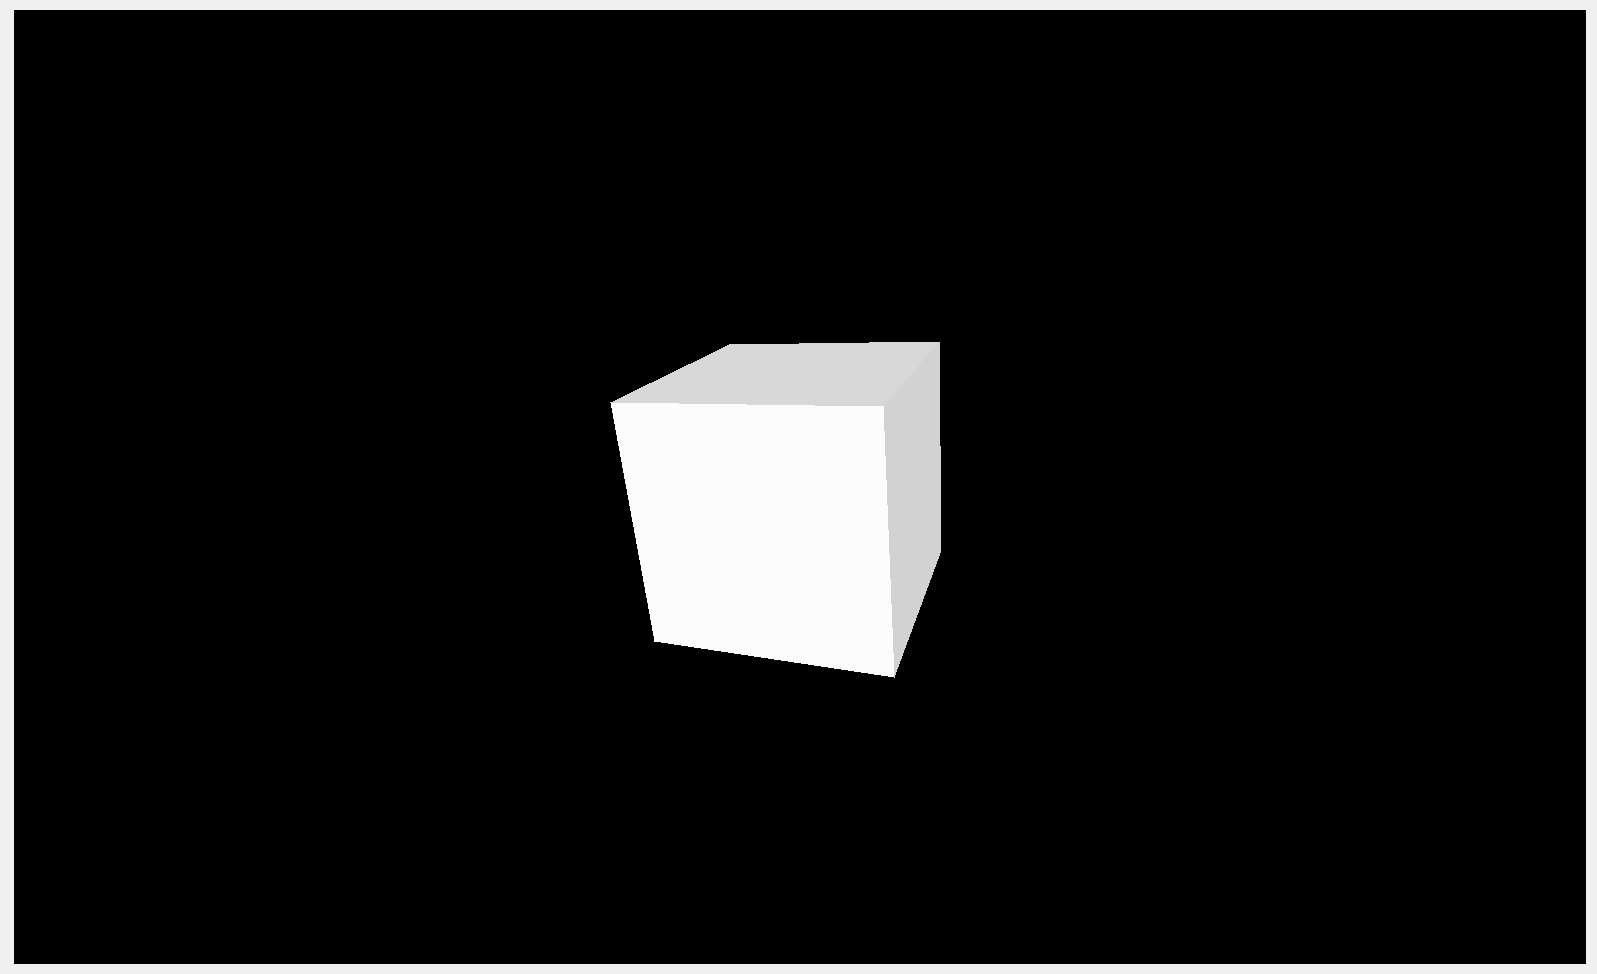
\includegraphics[scale=0.35]{screen}}
	\caption{Холст}
	\label{fig:screen}
\end{figure}

Интерфейс перемещения между группами интерфейса позволяет пользователю просматривать различные группы элементов интерфейса, относящиеся к определённым элементам программы для просмотра моделей. Реализован в виде двух кнопок, позволяющих просматривать пердыдущую и следующую группу элементов интерфейса. Ниже на рисунке \ref{fig:arrows} приведена реализация интерфейса перемещения в графическом интерфейсе программы для просмотра моделей.
\begin{figure}[H]
	\center{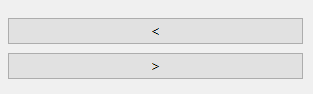
\includegraphics[scale=0.8]{arrows}}
	\caption{Интерфейс перемещения между группами интерфейса}
	\label{fig:arrows}
\end{figure}

Интейфейс параметров модели позволяет просматривать и изменять параметры модели, сохранять модель и загружать модели либо из объектного файла, либо из списка моделей. Ниже на рисунке \ref{fig:model_params} приведена реализация интерфейса параметров модели в графическом интерфейсе программы для просмотра моделей.
\begin{figure}[H]
	\center{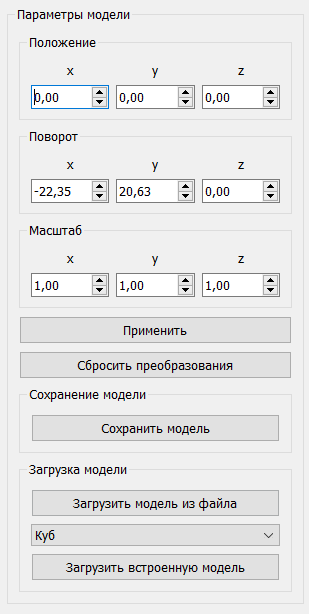
\includegraphics[scale=0.8]{model_params}}
	\caption{Интерфейс параметров модели}
	\label{fig:model_params}
\end{figure}

Интерфейс параметров камеры позволяет просматривать и изменять параметры виртуальной камеры. Ниже на рисунке \ref{fig:model_params} приведена реализация интерфейса параметров камеры в графическом интерфейсе программы для просмотра моделей.
\begin{figure}[H]
	\center{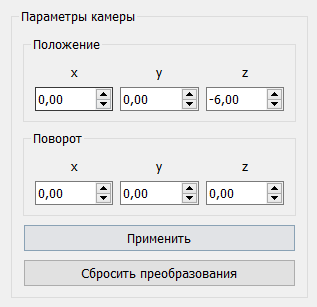
\includegraphics[scale=0.8]{camera_params}}
	\caption{Интерфейс параметров виртуальной камеры}
	\label{fig:model_params}
\end{figure}

Интейрфейс параметров освещения позволяет просматривать и изменять параметры источника освещения. Ниже на рисунке \ref{fig:light_params} приведена реализация интерфейса параметров освещения в графическом интерфейсе редактора.
\begin{figure}[H]
	\center{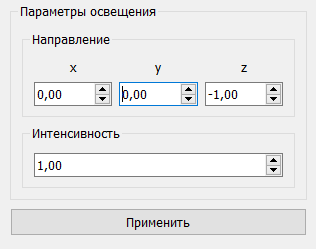
\includegraphics[scale=1.0]{light_params}}
	\caption{Интерфейс параметров освещения}
	\label{fig:light_params}
\end{figure}

Интейрфейс параметров освещения позволяет создавать снимок сцены и сохранять его в виде файла формата png. Ниже на рисунке \ref{fig:render_params} приведена реализация интерфейса синтеза изображения графическом интерфейсе программы для просмотра моделей.
\begin{figure}[H]
	\center{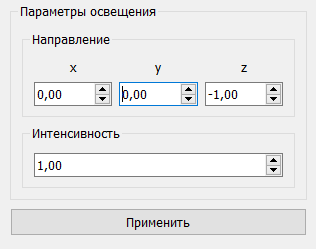
\includegraphics[scale=1.0]{light_params}}
	\caption{Интерфейс синтеза изображения}
	\label{fig:render_params}
\end{figure}

Интерфейс сопределения наиболее вероятного соответствия объекта, изображённого на двумерном снимке загружать файл с изображением трёхмерного объекта для определения модели из списка моделей, которая наиболее вероятно изображена на загруженном изображении. Ниже на рисунке \ref{fig:recognize_params} приведена реализация данного интерфейса в графическом интерфейсе программы для просмотра моделей.
\begin{figure}[H]
	\center{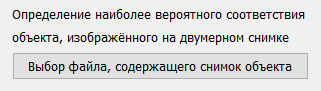
\includegraphics[scale=1.0]{recognize_params}}
	\caption{Интерфейс определения наиболее вероятного соответствия объекта, изображённого на двумерном снимке}
	\label{fig:recognize_params}
\end{figure}

\section{Вывод из технологического раздела}
В данном разделе был рассмотрен выбор языка программирования и среды разработки для проекта. Были представлены листинги реализаций основных алгоритмов, использованных при решении задачи. Были представлены сведения о модулях программы и информация, необходимая для сборки и запуска разработанного программного обеспечения. Был описан интерфейс разработанного программного обеспечения.